%package list
\documentclass{article}
\usepackage[top=3cm, bottom=3cm, outer=3cm, inner=3cm]{geometry}
\usepackage{multicol}
\usepackage{graphicx}
\usepackage{url}
%\usepackage{cite}
\usepackage{hyperref}
\usepackage{array}
%\usepackage{multicol}
\newcolumntype{x}[1]{>{\centering\arraybackslash\hspace{0pt}}p{#1}}
\usepackage{natbib}
\usepackage{pdfpages}
\usepackage{multirow}
\usepackage[normalem]{ulem}
\useunder{\uline}{\ul}{}
\usepackage{svg}
\usepackage{xcolor}
\usepackage{listings}

\lstdefinestyle{ascii-tree}{
    literate={├}{|}1 {─}{--}1 {└}{+}1 
  }
\lstset{basicstyle=\ttfamily,
  showstringspaces=false,
  commentstyle=\color{red},
  keywordstyle=\color{blue}
}
%\usepackage{booktabs}
\usepackage{caption}
\usepackage{subcaption}
\usepackage{float}
\usepackage{array}

\newcolumntype{M}[1]{>{\centering\arraybackslash}m{#1}}
\newcolumntype{N}{@{}m{0pt}@{}}


%%%%%%%%%%%%%%%%%%%%%%%%%%%%%%%%%%%%%%%%%%%%%%%%%%%%%%%%%%%%%%%%%%%%%%%%%%%%
%%%%%%%%%%%%%%%%%%%%%%%%%%%%%%%%%%%%%%%%%%%%%%%%%%%%%%%%%%%%%%%%%%%%%%%%%%%%
\newcommand{\itemEmail}{aphoccot@unsa.edu.pe}
\newcommand{\itemStudent}{Alejandro Josue Phocco Tapia}
\newcommand{\itemCourse}{Programación Web 2}
\newcommand{\itemCourseCode}{20220589}
\newcommand{\itemSemester}{III}
\newcommand{\itemUniversity}{Universidad Nacional de San Agustín de Arequipa}
\newcommand{\itemFaculty}{Facultad de Ingeniería de Producción y Servicios}
\newcommand{\itemDepartment}{Departamento Académico de Ingeniería de Sistemas e Informática}
\newcommand{\itemSchool}{Escuela Profesional de Ingeniería de Sistemas}
\newcommand{\itemAcademic}{2023 - A}
\newcommand{\itemInput}{Del 08 Mayo 2023}
\newcommand{\itemOutput}{Al 15 Junio 2023}
\newcommand{\itemPracticeNumber}{05}
\newcommand{\itemTheme}{Python - Django}
%%%%%%%%%%%%%%%%%%%%%%%%%%%%%%%%%%%%%%%%%%%%%%%%%%%%%%%%%%%%%%%%%%%%%%%%%%%%
%%%%%%%%%%%%%%%%%%%%%%%%%%%%%%%%%%%%%%%%%%%%%%%%%%%%%%%%%%%%%%%%%%%%%%%%%%%%

\usepackage[english,spanish]{babel}
\usepackage[utf8]{inputenc}
\AtBeginDocument{\selectlanguage{spanish}}
\renewcommand{\figurename}{Figura}
\renewcommand{\refname}{Referencias}
\renewcommand{\tablename}{Tabla} %esto no funciona cuando se usa babel
\AtBeginDocument{%
	\renewcommand\tablename{Tabla}
}

\usepackage{fancyhdr}
\pagestyle{fancy}
\fancyhf{}
\setlength{\headheight}{30pt}
\renewcommand{\headrulewidth}{1pt}
\renewcommand{\footrulewidth}{1pt}
\fancyhead[L]{\raisebox{-0.2\height}{
\includegraphics[width=3cm]{img/logo_episunsa.png}}}
\fancyhead[C]{\fontsize{7}{7}\selectfont	\itemUniversity \\ \itemFaculty \\ \itemDepartment \\ \itemSchool \\ \textbf{\itemCourse}}
\fancyhead[R]{\raisebox{-0.2\height}{
\includegraphics[width=1.2cm]{img/logo_abet}}}
\fancyfoot[L]{Estudiante Alejandro Phocco Tapia}
\fancyfoot[C]{\itemCourse}
\fancyfoot[R]{Página \thepage}

% para el codigo fuente
\usepackage{listings}
\usepackage{color, colortbl}
\definecolor{dkgreen}{rgb}{0,0.6,0}
\definecolor{gray}{rgb}{0.5,0.5,0.5}
\definecolor{mauve}{rgb}{0.58,0,0.82}
\definecolor{codebackground}{rgb}{0.95, 0.95, 0.92}
\definecolor{tablebackground}{rgb}{0.8, 0, 0}

\lstset{frame=tb,
	language=bash,
	aboveskip=3mm,
	belowskip=3mm,
	showstringspaces=false,
	columns=flexible,
	basicstyle={\small\ttfamily},
	numbers=none,
	numberstyle=\tiny\color{gray},
	keywordstyle=\color{blue},
	commentstyle=\color{dkgreen},
	stringstyle=\color{mauve},
	breaklines=true,
	breakatwhitespace=true,
	tabsize=3,
	backgroundcolor= \color{codebackground},
}

\begin{document}
	
	\vspace*{10px}
	
	\begin{center}	
		\fontsize{17}{17} \textbf{ Informe de Laboratorio \itemPracticeNumber}
	\end{center}
	\centerline{\textbf{\Large Tema: \itemTheme}}
	%\vspace*{0.5cm}	

	\begin{flushright}
		\begin{tabular}{|M{2.5cm}|N|}
			\hline 
			\rowcolor{tablebackground}
			\color{white} \textbf{Nota}  \\
			\hline 
			     \\[30pt]
			\hline 			
		\end{tabular}
	\end{flushright}	

	\begin{table}[H]
		\begin{tabular}{|x{4.7cm}|x{4.8cm}|x{4.8cm}|}
			\hline 
			\rowcolor{tablebackground}
			\color{white} \textbf{Estudiante} & \color{white}\textbf{Escuela}  & \color{white}\textbf{Asignatura}   \\
			\hline 
			{\itemStudent \par \itemEmail} & \itemSchool & {\itemCourse \par Semestre: \itemSemester \par Código: \itemCourseCode}     \\
			\hline 			
		\end{tabular}
	\end{table}		
	
	\begin{table}[H]
		\begin{tabular}{|x{4.7cm}|x{4.8cm}|x{4.8cm}|}
			\hline 
			\rowcolor{tablebackground}
			\color{white}\textbf{Laboratorio} & \color{white}\textbf{Tema}  & \color{white}\textbf{Duración}   \\
			\hline 
			\itemPracticeNumber & \itemTheme & 04 horas   \\
			\hline 
		\end{tabular}
	\end{table}
	
	\begin{table}[H]
		\begin{tabular}{|x{4.7cm}|x{4.8cm}|x{4.8cm}|}
			\hline 
			\rowcolor{tablebackground}
			\color{white}\textbf{Semestre académico} & \color{white}\textbf{Fecha de inicio}  & \color{white}\textbf{Fecha de entrega}   \\
			\hline 
			\itemAcademic & \itemInput &  \itemOutput  \\
			\hline 
		\end{tabular}
	\end{table}
	
	\section{Tarea}
	\begin{itemize}		
		\item Crea un blog sencillo en un entorno virtual utilizando la guía: \url{https://tutorial.djangogirls.org/es/django_start_project/}
            \item Especificar paso a paso la creación del blog en su informe.
	\end{itemize}
        \begin{figure}[H]
		\centering
		
\includegraphics[width=0.25\textwidth,keepaspectratio]{img/django.png}
	\end{figure}

	\section{URL de Repositorio Github}
	\begin{itemize}
		\item URL para el laboratorio 05 en el Repositorio GitHub.
		\item \url{https://github.com/AlejandroPhoccoTapia/Lab05-PW2-AlejandroPhocco}
	\end{itemize}
	
	\section{Ejercicios}
 
 
	\subsection{Análisis de archivos }
 
        
	\begin{lstlisting}[language=bash,caption={Analizando bloque 1 de settings.py}][H]
            INSTALLED_APPS = [
                'django.contrib.admin',
                'django.contrib.auth',
                'django.contrib.contenttypes',
                'django.contrib.sessions',
                'django.contrib.messages',
                'django.contrib.staticfiles',
                'Blog'
            ]
	\end{lstlisting}
        Estas son las configuraciones de las aplicaciones instaladas, la ultima aplicacion "blog" es la que creamos para nuestro blog personal.
        
        \begin{itemize}	
    		\item Veremos el archivo models.py de la app Blog
        \end{itemize}
        \begin{lstlisting}[language=bash,caption={bloque4}][H]
        from django.db import models
        from django.utils import timezone
        
        # Create your models here.
        
        class Post(models.Model):
            title = models.CharField(max_length = 200)
            text = models.TextField()
            create_date = models.DateTimeField(default=timezone.now)
            published_date = models.DateTimeField(blank=True, null=True)
        
            def __str__(self):
                return self.title
	\end{lstlisting}
    
    Veamos que se tienen los atributos title, text, created\_date  y created\_date para definir sus respectivos aspectos: un titulo y texto a ingresar, la hora de creacion y la hora de publicacion. Ademas tenemos un Metodo que devolvera el titulo del post.

        \begin{itemize}	
    		\item Archivo admin
        \end{itemize}
        
        \begin{lstlisting}[language=bash,caption={admin.py}][H]
            from django.contrib import admin
            from .models import Post
            
            # Register your models here.
            
            admin.site.register(Post)
	\end{lstlisting}
    Agregamos el modelo Post al admin de Blog para que Django se encargue de crearlo en la base de datos.   

        \begin{itemize}	
    		\item Archivo urls
        \end{itemize}
        
        \begin{lstlisting}[language=bash,caption={urls.py}][H] 
            from django.urls import path
            from . import views
            
            urlpatterns = [
                path('', views.index, name = 'index'),
                path('new_post/', views.newPost, name = "new_post" ),
                path('post/<int:id>', views.post, name = "post"),
                path('edit_post/<int:id>', views.editPost, name = "edit_post"),
                path('delete_post/<int:id>', views.deletePost, name = "delete_post")
            ]
	\end{lstlisting}
    Estas son las rutas que usaremos en el blog la primera siendo la pagina principal, la segunda para crear un nuevo post, la tercera para revisar la informacion de un post en especifico, la cuarta para editar un post en especifico y la quinta para borrar un post en especifico.

	\begin{itemize}	
		\item Archivos views
	\end{itemize}
	\begin{lstlisting}[language=bash,caption={views.py}][H]
            from django.shortcuts import render, redirect
            from .models import Post
            from .forms import CreateNewPost
            from django.utils import timezone
            
            # Create your views here.
            
            def index(request):
                posts = list(Post.objects.order_by('-published_date'))
                return render(request, 'index.html', {'posts': posts})
            
            def newPost(request):
                if request.method == 'GET':
                    return render(request, 'newPost.html', {'form': CreateNewPost()})
                else:
                    Post.objects.create(title=request.POST['title'], text=request.POST['text'], published_date=timezone.now())
                    return redirect('/')
            
            def post(request, id):
                post = Post.objects.get(id=id)
                return render(request, 'post.html', {'post': post})
            
            def editPost(request, id):
                if request.method == 'GET':
                    post = Post.objects.get(id=id)
                    form = CreateNewPost(instance=post)
                    return render(request, 'editPost.html', {'form' : form})
                else:
                    post = Post.objects.get(id=id)
                    post.published_date = timezone.now()
                    form = CreateNewPost(request.POST, instance=post)
                    if form.is_valid():
                        form.save()
                        return redirect('/')
            
            def deletePost(request, id):
                post = Post.objects.get(id=id)
                post.delete()
                return redirect('/')
	\end{lstlisting}
        Aqui vemos que cada metodo se encarga de renderizar su respectivo html y algunos dependiendo de si utilizan el metodo get o post para acceder a ellos hacen algunos cosas distintas.

        \begin{itemize}	
		\item Plantilas HTML 
	\end{itemize}
	\begin{lstlisting}[language=bash,caption={index.html}][H]
            

            <!DOCTYPE html>
            <html lang="en">
              <head>
                <meta charset="UTF-8" />
                <meta name="viewport" content="width=device-width, initial-scale=1.0" />
                <link rel="stylesheet" href="" />
                <title>Document</title>
              </head>
              <body>
                <header class="header">
                  <h1 class="header__h1">Mi Blog Personal</h1>
                  <a href="" class="header__a">Añadir</a>
                </header>
            
                <main class="main">
                  
            
                  <article class="article">
                    <h2 class="article__h2">
                      <a href="" class="article__a"
                        >{{ post.title }}</a
                      >
                    </h2>
                    <p class="article__p">{{ post.text }}</p>
                  </article>
            
                  
                </main>
              </body>
            </html>
	\end{lstlisting}
        Este es el html de la pagina principal del blog como vemos Django se encarga de prepocesar este archivo utilizando un lenguaje incluido en el archivo.

        \begin{lstlisting}[language=bash,caption={newPost.html}][H]
            

            <!DOCTYPE html>
            <html lang="en">
              <head>
                <meta charset="UTF-8" />
                <meta name="viewport" content="width=device-width, initial-scale=1.0" />
                <link rel="stylesheet" href="" />
                <title>Document</title>
              </head>
              <body>
                <header class="header">
                  <h1 class="header__h1">Mi Blog Personal</h1>
                </header>
            
                <main class="main">
                  <form method="post">
                     {{ form }}
                    <button>Enviar</button>
                  </form>
                </main>
              </body>
            </html>
	\end{lstlisting}
        Esta plantilla es la que se encarga de mostrar el formulario para crear un nuevo Post.

        \begin{lstlisting}[language=bash,caption={post.html}][H]
            

            <!DOCTYPE html>
            <html lang="en">
              <head>
                <meta charset="UTF-8" />
                <meta name="viewport" content="width=device-width, initial-scale=1.0" />
                <link rel="stylesheet" href="" />
                <title>Document</title>
              </head>
              <body>
                <header class="header">
                  <h1 class="header__h1">Mi Blog Personal</h1>
                </header>
            
                <main class="main">
                  <article class="article">
                    <h5 class="article__h5">{{ post.create_date }}</h5>
                    <a href="">Editar</a>
                    <a href="">Eliminar</a>
                    <h2 class="article__h2">
                      <a href="" class="article__a">{{ post.title }}</a>
                    </h2>
                    <p class="article__p">{{ post.text }}</p>
                  </article>
                </main>
              </body>
            </html>
	\end{lstlisting}
         Esta plantilla se encarga de mostrar los detalles de un post.

         \begin{lstlisting}[language=bash,caption={editPost.html}][H]
            

            <!DOCTYPE html>
            <html lang="en">
              <head>
                <meta charset="UTF-8" />
                <meta name="viewport" content="width=device-width, initial-scale=1.0" />
                <link rel="stylesheet" href="" />
                <title>Document</title>
              </head>
              <body>
                <header class="header">
                  <h1 class="header__h1">Mi Blog Personal</h1>
                </header>
            
                <main class="main">
                  <form method="post">
                     {{ form }}
                    <button>Enviar</button>
                  </form>
                </main>
              </body>
            </html>
	\end{lstlisting}
        Esta plantilla se encarga de generar un form para editar un post.

        \item \textbf{Archivos de estilos, blogs.css}
        \begin{lstlisting}[language=bash,caption={style.css}][H]
            body {
              padding: 0;
              margin: 0;
              min-height: 100vh;
              display: flex;
              flex-direction: column;
            }
            
            .header {
              background-image: linear-gradient(to right, hsl(45 100% 65%), hsl(25 100% 45%));
              height: 5rem;
              position: relative;
            }
            
            .header__h1 {
              margin: 1rem 0 0 1rem;
            }
            
            .header__a {
              display: block;
              background-color: hsl(0 0% 100%);
              width: 5rem;
              height: 2rem;
              text-decoration: none;
              position: absolute;
              right: 1rem;
              top: 1.5rem;
              color: hsl(0 0% 0%);
              display: flex;
              align-items: center;
              justify-content: center;
              border-radius: 0.5rem;
              transition: background-color 100ms, color 100ms;
            }
            
            .header__a:hover {
              color: hsl(0 0% 100%);
              background-color: hsl(25 100% 45%);
            }
            
            .main {
              background-color: hsl(0 0% 90%);
              height: 100%;
              flex-grow: 1;
            }
            
            .article {
              padding: 1rem 1rem;
              overflow-wrap: break-word;
            }
            
            .article__h2 {
              margin: 0;
            }
            
            .article__a {
              text-decoration: none; 
              color: hsl(0 0% 0%);
            } 
            
            .article__p {
              margin: 0;
              text-overflow: clip;
            }
	\end{lstlisting}
        Este es el archivo css que les dara estilos a neustros anteriores html.

        \item \textbf{Archivo forms}
        \begin{lstlisting}[language=bash,caption={forms.py}][H]
            from django import forms
            from .models import Post
            
            class CreateNewPost(forms.ModelForm):
                
            
                class Meta:
                    model = Post
                    fields = ['title', 'text',]
	\end{lstlisting}
        Esta clase CreateNewPost es un formulario que toma como base el modelo Post pero teniendo como campos solo el titulo y el texto del mismo.\newline\newline
        \subsection{Ejecucion}
        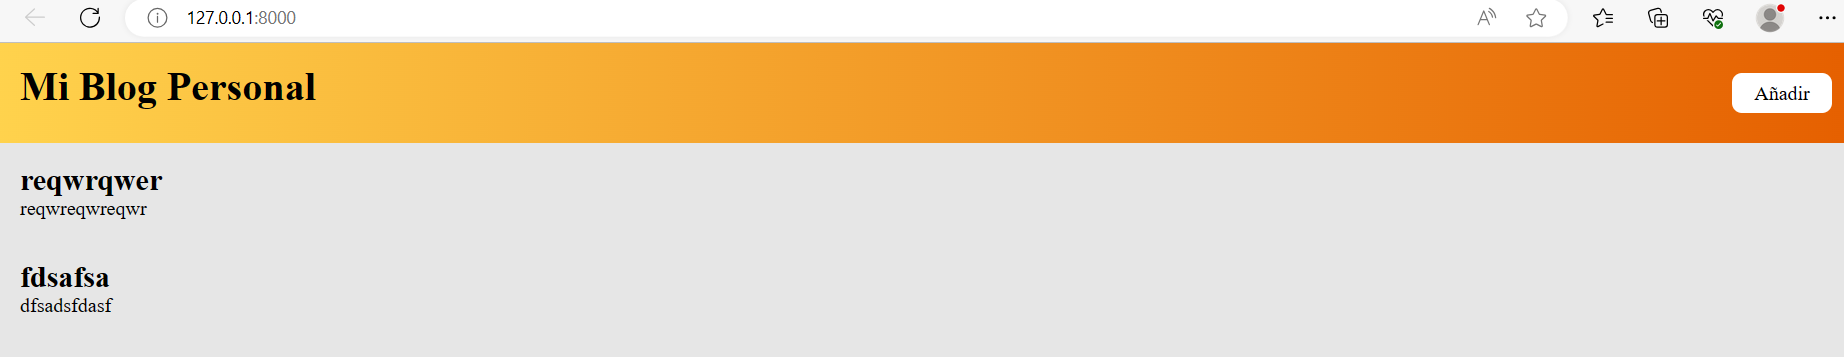
\includegraphics[width=16cm]{img/ejecucion1.png}
        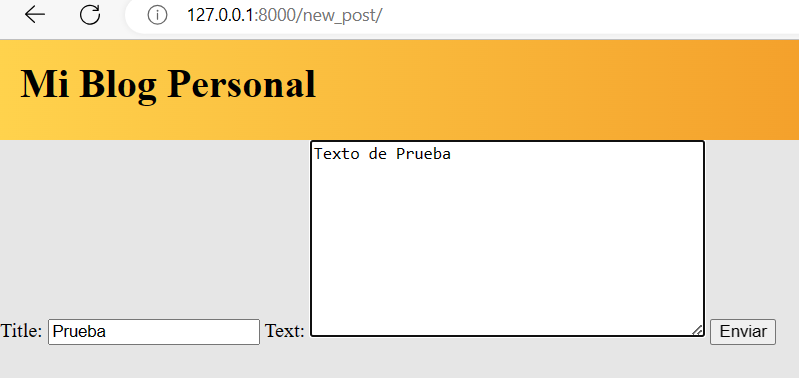
\includegraphics[width=16cm]{img/ejecucion2.png}
        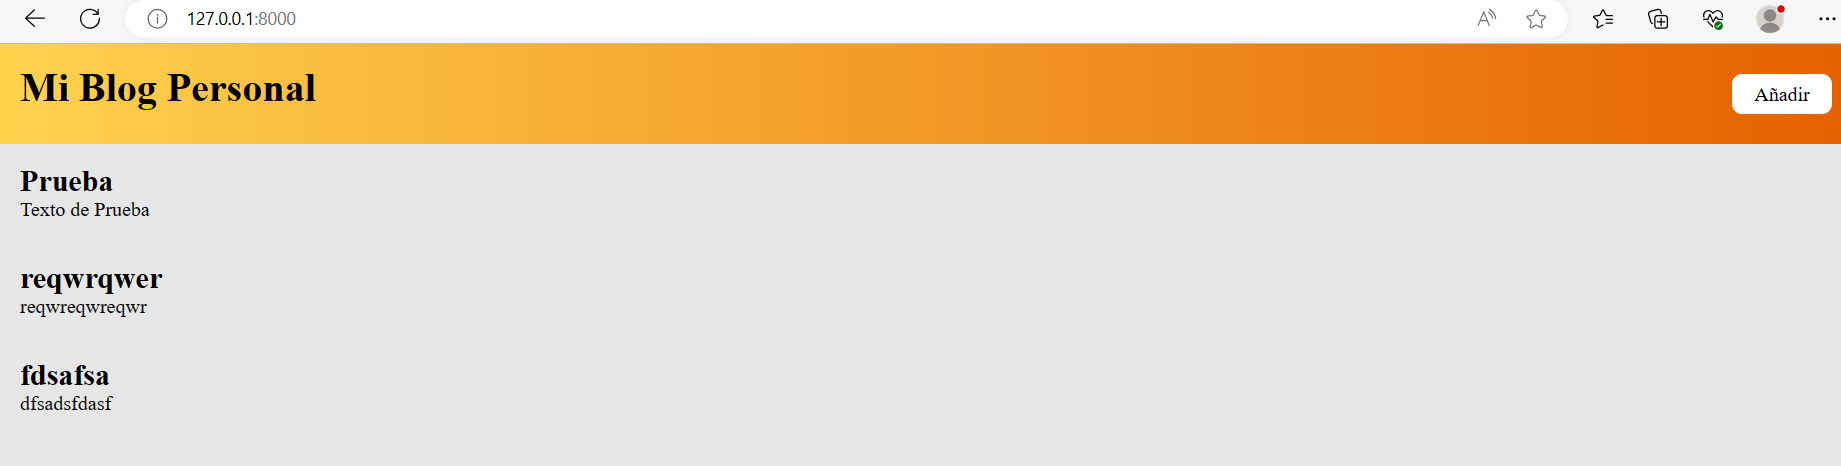
\includegraphics[width=16cm]{img/ejecucion3.png}
        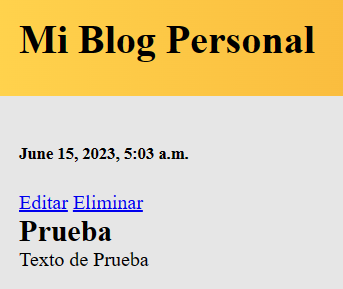
\includegraphics[width=16cm]{img/ejecucion4.png}
        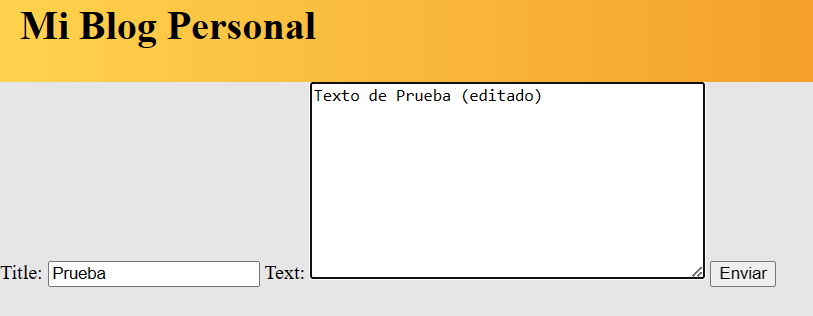
\includegraphics[width=16cm]{img/ejecucion5.png}
        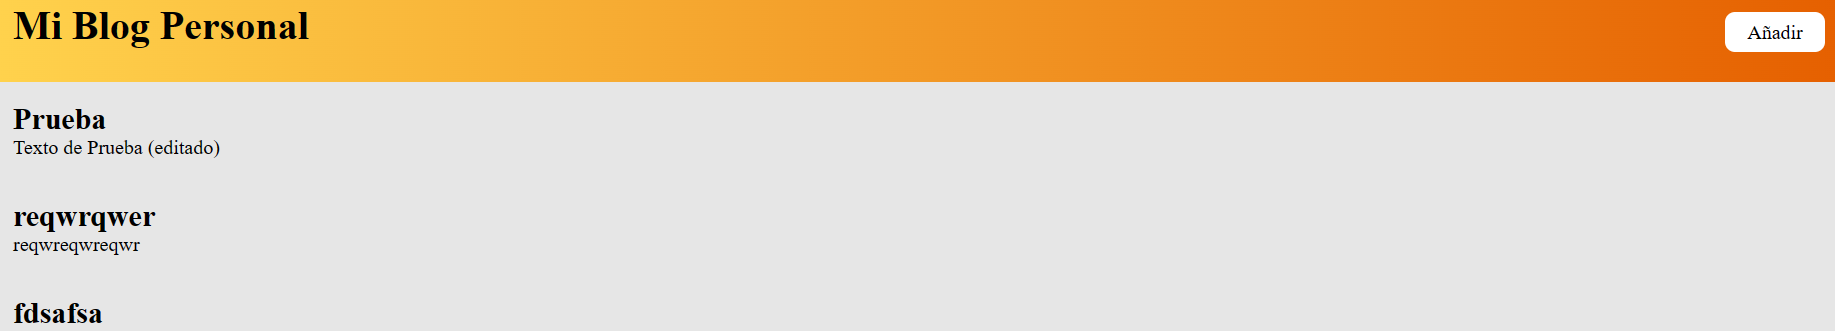
\includegraphics[width=16cm]{img/ejecucion6.png}
        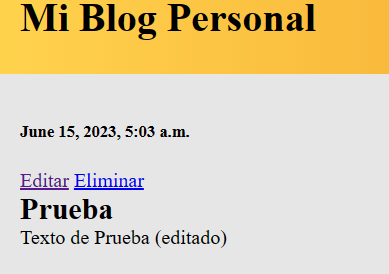
\includegraphics[width=16cm]{img/ejecucion7.png}
        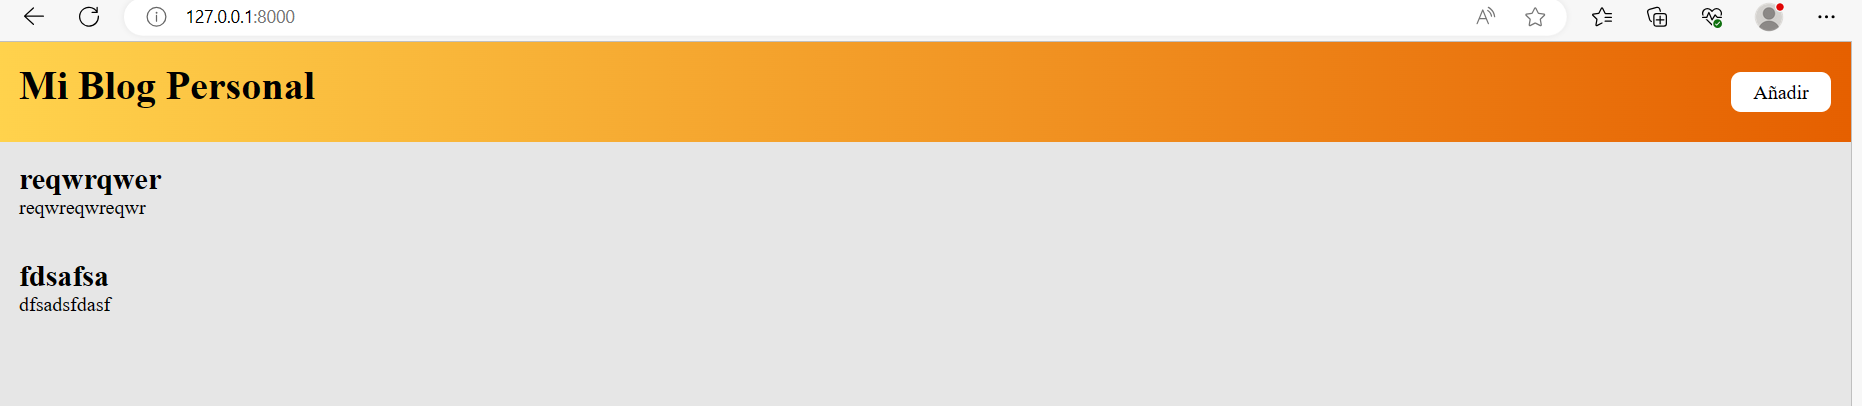
\includegraphics[width=16cm]{img/ejecucion8.png}
        
        
\section{Cuestionario}
	\begin{itemize}
		\item{¿Cuál es un estándar de codificación para Python? Ejemplo: Para PHP en el proyecto Pear \url{https://pear.php.net/manual/en/standards.php}}
        Uno de los estándares de codificación más ampliamente aceptados y utilizados en Python se conoce como PEP 8 (Python Enhancement Proposal 8). PEP 8 establece una guía de estilo para escribir código Python con el fin de mejorar la legibilidad del codigo y llegar a un estandar para el codigo de python.\newline

		\item{¿Qué diferencias existen entre EasyInstall, pip, y PyPM?}\newline
        EasyInstall fue uno de los primeros administradores de paquetes de Python, pero actualmente su uso es muy escaso. Pip es el administrados de paquetes por excelencia actualmente. PyPM es un administrador de paquetes para ActivePython, pero ya no recibe actualizaciones y se recomienda usar pip.  \newline

\item{En un proyecto Django que se debe ignorar para usar git. Vea: \url{https://github.com/django/django/blob/main/.gitignore}. ¿Qué otros tipos de archivos se deberían agregar a este archivo?}\newline
  Se debe ignorar los archivos del entorno virtual, los datos de la base de datos, las migraciones y los archivos generados por python a la hora de compilar.
  
	\end{itemize}	
 \newpage
 \section{Conclusiones}
	\begin{itemize}
    Django es un framework bastante potente que permite poder crear una aplicacion con buena seguridad, flexible y de alto nivel.
	\end{itemize}	
\clearpage

\section{Referencias}
\begin{itemize}	
    \item \url{https://www.w3schools.com/python/python_reference.asp}
    \item \url{ https://docs.python.org/3/tutorial/}
    \item \url{https://developer.mozilla.org/es/docs/Learn/Server-side/Django/Models}
    \item \url{https://tutorial.djangogirls.org/es/django_models/}
    \item \url{https://pear.php.net/manual/en/standards.php}
    \item \url{https://docs.djangoproject.com/en/4.0/}
    \item \url{https://www.youtube.com/watch?v=M4NIs4BM1dk}
    \item \url{https://pypi.org/}
    \item \url{https://pip.pypa.io/en/latest/user_guide/}
    \item \url{https://packaging.python.org/en/latest/tutorials/installing-packages/}
\end{itemize}	
	
%\clearpage
%\bibliographystyle{apalike}
%\bibliographystyle{IEEEtranN}
%\bibliography{bibliography}
			
\end{document}